\section{First Member}
This is the section dedicated to one of the team members, and it should be written individually . It can include a range of things; first subsection is a space for you to point out the strengths and weaknesses of the module, including complaints about the module coordinator Max Wilson. The second section should have a selfie image with Max! The last part of it is the most important one. You will need to write a paragraph about what you have learned in this module. You can write it in \textbf{Bold} if you want or you can use other fonts. 

Please do not forget:
\begin{itemize}
	\item First paragraph should have your comments about the module
	\item Second one, a picture img of Max
	\item Last one, what you learned in this module.
\end{itemize}

\subsection{Comments about the module}
Hello my name is \textsc{naqeeb} \textcolor{blue}{and} \textcolor{red}{i} \textcolor{green}{have} learnt a bit in this module. Max is ok.

\subsection{Picture of Max}


\begin{figure}[h]
\caption{Max Wilson (googled him)}
\centering
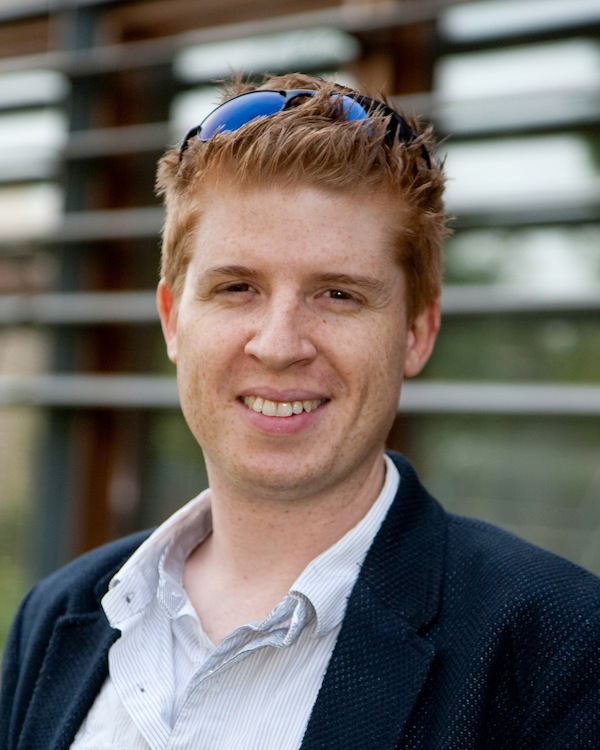
\includegraphics[width=0.5\textwidth]{max.jpg}
\label{fig:Max}
\end{figure}

%You can then use the label of the figure to reference it later with the command ${\backslash}ref$. you can comment out the next line to see an example of how it works.

My Picture of Max is in  Figure \ref{fig:Max}.

\subsection{What I have learned in this module}
About
\begin{itemize}
	\item Personas,
	\item UML Diagrams,
	\item Software Engineering,
	\item Google,
	\item Apple,
	\item Max's dress sense,
	\item How to put images into LateX projects,
	\item How to set up a GitHub profile and start a git project.
\end{itemize}

